\newcommand{\svrname}{Dr John Fawcett}
\newcommand{\jkfside}{oneside}
\newcommand{\jkfhanded}{right}

\newcommand{\studentname}{Harry Langford}
\newcommand{\studentemail}{hjel2@cam.ac.uk}

\documentclass[10pt,\jkfside,a4paper]{article}

\newcommand{\svcourse}{CST Part IA: Software Engineering and Security}
\newcommand{\svnumber}{1}
\newcommand{\svvenue}{Microsoft Teams}
\newcommand{\svdate}{2022-05-11}
\newcommand{\svtime}{15:00}
\newcommand{\svuploadkey}{CBd13xmL7PC1zqhNIoLdTiYUBnxZhzRAtJxv/ytRdM1r7qIfwMsxeVwM/pPcIo8l}

\newcommand{\svrname}{Dr Sam Ainsworth}
\newcommand{\jkfside}{oneside}
\newcommand{\jkfhanded}{yes}

\newcommand{\studentname}{Harry Langford}
\newcommand{\studentemail}{hjel2@cam.ac.uk}

% DO NOT add \usepackage commands here.  Place any custom commands
% into your SV work files.  Anything in the template directory is
% likely to be overwritten!

\usepackage{fancyhdr}

\usepackage{lastpage}       % ``n of m'' page numbering
\usepackage{lscape}         % Makes landscape easier

\usepackage{verbatim}       % Verbatim blocks
\usepackage{listings}       % Source code listings
\usepackage{epsfig}         % Embed encapsulated postscript
\usepackage{array}          % Array environment
\usepackage{qrcode}         % QR codes
\usepackage{enumitem}       % Required by Tom Johnson's exam question header

\usepackage{hhline}         % Horizontal lines in tables
\usepackage{siunitx}        % Correct spacing of units
\usepackage{amsmath}        % American Mathematical Society
\usepackage{amssymb}        % Maths symbols
\usepackage{amsthm}         % Theorems

\usepackage{ifthen}         % Conditional processing in tex

\usepackage[top=3cm,
            bottom=3cm,
            inner=2cm,
            outer=5cm]{geometry}

% PDF metadata + URL formatting
\usepackage[
            pdfauthor={\studentname},
            pdftitle={\svcourse, SV \svnumber},
            pdfsubject={},
            pdfkeywords={9d2547b00aba40b58fa0378774f72ee6},
            pdfproducer={},
            pdfcreator={},
            hidelinks]{hyperref}


% DO NOT add \usepackage commands here.  Place any custom commands
% into your SV work files.  Anything in the template directory is
% likely to be overwritten!

\usepackage{fancyhdr}

\usepackage{lastpage}       % ``n of m'' page numbering
\usepackage{lscape}         % Makes landscape easier

\usepackage{verbatim}       % Verbatim blocks
\usepackage{listings}       % Source code listings
\usepackage{graphicx}
\usepackage{float}
\usepackage{epsfig}         % Embed encapsulated postscript
\usepackage{array}          % Array environment
\usepackage{qrcode}         % QR codes
\usepackage{enumitem}       % Required by Tom Johnson's exam question header

\usepackage{hhline}         % Horizontal lines in tables
\usepackage{siunitx}        % Correct spacing of units
\usepackage{amsmath}        % American Mathematical Society
\usepackage{amssymb}        % Maths symbols
\usepackage{amsthm}         % Theorems

\usepackage{ifthen}         % Conditional processing in tex

\usepackage[top=3cm,
            bottom=3cm,
            inner=2cm,
            outer=5cm]{geometry}

% PDF metadata + URL formatting
\usepackage[
            pdfauthor={\studentname},
            pdftitle={\svcourse, SV \svnumber},
            pdfsubject={},
            pdfkeywords={9d2547b00aba40b58fa0378774f72ee6},
            pdfproducer={},
            pdfcreator={},
            hidelinks]{hyperref}

\renewcommand{\headrulewidth}{0.4pt}
\renewcommand{\footrulewidth}{0.4pt}
\fancyheadoffset[LO,LE,RO,RE]{0pt}
\fancyfootoffset[LO,LE,RO,RE]{0pt}
\pagestyle{fancy}
\fancyhead{}
\fancyhead[LO,RE]{{\bfseries \studentname}\\\studentemail}
\fancyhead[RO,LE]{{\bfseries \svcourse, SV~\svnumber}\\\svdate\ \svtime, \svvenue}
\fancyfoot{}
\fancyfoot[LO,RE]{For: \svrname}
\fancyfoot[RO,LE]{\today\hspace{1cm}\thepage\ / \pageref{LastPage}}
\fancyfoot[C]{\qrcode[height=0.8cm]{\svuploadkey}}
\setlength{\headheight}{22.55pt}


\ifthenelse{\equal{\jkfside}{oneside}}{

 \ifthenelse{\equal{\jkfhanded}{left}}{
  % 1. Left-handed marker, one-sided printing or e-marking, use oneside and...
  \evensidemargin=\oddsidemargin
  \oddsidemargin=73pt
  \setlength{\marginparwidth}{111pt}
  \setlength{\marginparsep}{-\marginparsep}
  \addtolength{\marginparsep}{-\textwidth}
  \addtolength{\marginparsep}{-\marginparwidth}
 }{
  % 2. Right-handed marker, one-sided printing or e-marking, use oneside.
  \setlength{\marginparwidth}{111pt}
 }

}{
 % 3. Alternating margins, two-sided printing, use twoside.
}


\setlength{\parindent}{0em}
\addtolength{\parskip}{1ex}

% Exam question headings, labels and sensible layout (courtesy of Tom Johnson)
\setlist{parsep=\parskip, listparindent=\parindent}
\newcommand{\examhead}[3]{\section{#1 Paper #2 Question #3}}
\newenvironment{examquestion}[3]{
\examhead{#1}{#2}{#3}\setlist[enumerate, 1]{label=(\alph*)}\setlist[enumerate, 2]{label=(\roman*)}
\marginpar{\href{https://www.cl.cam.ac.uk/teaching/exams/pastpapers/y#1p#2q#3.pdf}{\qrcode{https://www.cl.cam.ac.uk/teaching/exams/pastpapers/y#1p#2q#3.pdf}}}
\marginpar{\footnotesize \href{https://www.cl.cam.ac.uk/teaching/exams/pastpapers/y#1p#2q#3.pdf}{https://www.cl.cam.ac.uk/\\teaching/exams/pastpapers/\\y#1p#2q#3.pdf}}
}{}


\usepackage{graphicx}
\graphicspath{ {./images/} }
\usepackage{enumitem}
\usepackage{xcolor}
\usepackage{tikz}
\usetikzlibrary{tikzmark}

\begin{document}

\begin{enumerate}

\item Write a java function that creates an array-of-arrays to represent an n$\times$n 
identity matrix of floats.
\item Write another Java functin that transposes an n$\times$n matrix represented 
using an array-of-arrays. Your function should be in-place, i.e. use only O(1) space.

Implemented in ``nnarray.java''. The class is pasted below.

\begin{verbatim}
public class nnarray {

    private final float[][] matrix;
    private final int n;

    nnarray(int n){
        this.n = n;
        matrix = new float[n][n];
        for (int i = 0; i < n; i++){
            matrix[i][i] = 1;
        }
    }

    void transpose(){
        float t;
        for (int i = 0; i < n; i++){
            for (int j = i; j < n; j++){
                t = matrix[i][j];
                matrix[i][j] = matrix[j][i];
                matrix[j][i] = t;
            }
        }
    }
}
\end{verbatim}

\item \subsection*{4.2}
Draw some simple diagrams to illustrate what happens with each step of the following 
Java code in memory.

Before Line 1:
\begin{tabular}{c|r}
location & value\\
\hline
0 & \\
1 & \\
2 & \\
3 & \\
4 & \\
\end{tabular}

p is assigned. However, since the value of p is null, it does not point to 
anything (it has a null pointer).

After Line 1:
\begin{tabular}{c|r}
location & value\\
\hline
0 & p\\
1 & \\
2 & \\
3 & \\
4 & \\
\end{tabular}

p2 is assigned to a new person. So p2 references the memory address of this new person.

After Line 2:
\begin{tabular}{c|r}
location & value\\
\hline
0 & p\tikzmark{2p}\\
1 & p2\tikzmark{2p2}\\
2 & Person instance\tikzmark{2person1}\\
3 & \\
4 & \\
\end{tabular}
\begin{tikzpicture}[overlay, remember picture, shorten >=.5pt, shorten <=.5pt, transform canvas={yshift=.25\baselineskip}]
\draw [->] ({pic cs:2p2}) [bend left] to ({pic cs:2person1});
\end{tikzpicture}

p is then set to reference whatever p2 is referencing. So p references the memory address 
of the person (2).

After Line 3:
\begin{tabular}{c|r}
location & value\\
\hline
0 & p \tikzmark{3p}\\
1 & p2 \tikzmark{3p2}\\
2 & Person instance \tikzmark{3person1}\\
3 & \\
4 & \\
\end{tabular}
\begin{tikzpicture}[overlay, remember picture, shorten >=.5pt, shorten <=.5pt, transform canvas={yshift=.25\baselineskip}]
\draw [->] ({pic cs:3p}) [bend left] to ({pic cs:3person1});
\draw [->] ({pic cs:3p2}) [bend left] to ({pic cs:3person1});
\end{tikzpicture}

p2 is then reassigned to a new person. So the p2 now references a new person. However: 
p is unnaffected.

After Line 4:
\begin{tabular}{c|r}
location & value\\
\hline
0 & p\tikzmark{4p}\\
1 & p2\tikzmark{4p2}\\
2 & Person instance\tikzmark{4person1}\\
3 & Person instance\tikzmark{4person2}\\
4 & \\
\end{tabular}
\begin{tikzpicture}[overlay, remember picture, shorten >=.5pt, shorten <=.5pt, transform canvas={yshift=.25\baselineskip}]
\draw [->] ({pic cs:4p}) [bend left] to ({pic cs:4person1});
\draw [->] ({pic cs:4p2}) [bend left] to ({pic cs:4person2});
\end{tikzpicture}

p is set to reference null. So p's pointer is removed. Since there is nothing referencing 
the old person (2), it is marked as unused and will (hopefully) be garbage-collected.

After Line 5:
\begin{tabular}{c|r}
location & value\\
\hline
0 & p\tikzmark{5p}\\
1 & p2\tikzmark{5p2}\\
2 & Person instance\tikzmark{5person1}\\
3 & Person instance\tikzmark{5person2}\\
4 & \\
\end{tabular}
\begin{tikzpicture}[overlay, remember picture, shorten >=.5pt, shorten <=.5pt, transform canvas={yshift=.25\baselineskip}]
\draw [->] ({pic cs:5p2}) [bend left] to ({pic cs:5person2});
\end{tikzpicture}

\begin{verbatim}
1	Person p = null;
2	Person p2 = new Person();
3	p = p2;
4	p2 = new Person();
5	p = null;
\end{verbatim}

\subsection*{3.3}

\begin{enumerate}[label=(\alph*)]
\item Implemented in ``Vector2D.java''. The class is pasted below:

\begin{verbatim}
public class Vector2D {

    private float[] xy;

    Vector2D(){
        xy = new float[] {0, 0};
    }

    Vector2D(float[] vect){
        set(vect);
    }

    Vector2D(float x, float y){
        set(x, y);
    }

    void set(float[] vect){
        if (vect.length == 2){
            xy = new float[] {vect[0], vect[1]};
        }
        else{
            throw new IllegalArgumentException();
        }
    }

    void set(float x, float y){
        xy = new float[] {x, y};
    }

    float getx(){return xy[0];}

    float gety(){return xy[1];}

    float[] getxy(){return new float[] {xy[0], xy[1]};}

    void add(Vector2D v){
        xy[0] += v.getx();
        xy[1] += v.gety();
    }

    void subtract(Vector2D v){
        xy[0] -= v.getx();
        xy[1] -= v.gety();
    }

    float dot(Vector2D v){
        return xy[0] * v.getx() + xy[1] * v.gety();
    }

    float magnitude(){
        return (float) Math.sqrt(Math.pow(xy[0], 2) + Math.pow(xy[1], 2));
    }

    void normalise(){
        float magnitude = magnitude();
        xy[0] /= magnitude;
        xy[1] /= magnitude;
    }

    void scale(float n){
        xy[0] *= n;
        xy[1] *= n;
    }
}
\end{verbatim}

\item What changes would be needed to make it immutable?

To make it immutable you'd have to remove all the ``set'' methods, 
and change the add, subtract, scale and normalise methods to return the 
result rather 
than set the current vector to be the result.

\item Contrast the following prototypes for the addition method for both the (i) 
mutable and (ii) immutable versions.

\begin{itemize}
\item \begin{verbatim} public void add(Vector2D v)\end{verbatim}
\item \begin{verbatim} public Vector2D add(Vector2D v)\end{verbatim}
\item \begin{verbatim} public Vector2D add(Vector2D v1, Vector2D v2)\end{verbatim}
\item \begin{verbatim} public static Vector2D add(Vector2D v1, Vector2D)\end{verbatim}
\end{itemize}

\begin{enumerate}[label=(\roman*)]

\item mutable:

The first signature is suited to a mutable Vector2D. It would suggest that the 
second vector is being added to the second and the result is being stored in the 
vector.

The second signature is less suitable for a mutable vector. The 
best mutable interpretation of 
this would be to add the second vector to the first and then return a new vector with 
the value of the old vector (so that the previous value is not lost). In practical 
terms there are few cases where you would 
want the old vector (and so this interpretation would be niche) -- 
conversely it could be argued that this implementation would  
be more flexible than the first implementation.

The third signature is not suitable to a mutable vector. This implies adding two 
vectors together and then returning the sum -- which is not a helpful 
implementation for an instance of vector.

The fourth signature is generally unsuitable to a mutable vector.  However, 
it is static so not specific to a vector and 
since it takes different arguments to more conventional add methods, it 
could overload add -- such an implementation could be useful for a mutable 
vector.

\item immutable:

The first signature is totally unsuitable to an immutable vector. Since there 
is no return type and the vector is immutable; this function can neither 
change variables or return variables and so can do nothing.

The second signature is suitable for an immutable vector. It allows the second vector 
to be added to the first and the result to be returned.

The third signature is not suited to an immutable vector. Adding two vectors 
together in an instance of a vector doesn't make sense.

The fourth signature is suited to an immutable vector. This is a static method 
and so specific to the class rather than an object. This means you would add 
together two vectors in the class rather than add one vector to another.

\end{enumerate}

\item How can you convey to a user of your class that it is immutable?

\begin{itemize}
\item You can make every function return a value -- to make it clear that none 
of them make any persistent changes.
\item You could include immutable in the name of the class.
\item Don't implement any methods which are ambigious -- ie which could be percieved 
to be mutable (ie ``update'').
\item You can include comments and documentation saying it is immutable.
\end{itemize}

\end{enumerate}

\subsection*{3.4}
\begin{enumerate}[label=(\alph*)]
\item Implemented in ``OOPLinkedList.java''. The class is pasted below.

\begin{verbatim}
package uk.ac.cam.hjel2.OOPsv1.LinkedList;
public class OOPLinkedList {

    OOPLinkedListElement head;
    int length;

    static class OOPLinkedListElement{

        final int value;
        OOPLinkedListElement next;

        OOPLinkedListElement(int v, OOPLinkedListElement pointer){
            value = v;
            next = pointer;
        }
    }

    public void add(int n){
        head = new OOPLinkedListElement(n, head);
        length += 1;
    }

    public void remove(){
        if (length != 0) {
            head = head.next;
            length -= 1;
        }
    }

    public int nth(int n){
        if (n >= length){
            throw new IndexOutOfBoundsException();
        }
        OOPLinkedListElement ith = head;
        for (int i = 0; i < n; i++){
            ith = head.next;
        }
        return ith.value;
    }

    public int head(){
        if (head != null){
            return head.value;
        }
        throw new IndexOutOfBoundsException("OOPLinkedList is empty");
    }

    public int length(){return length;}

    @Override
    public String toString(){
        OOPLinkedListElement current = head;
        if (current == null){return "[]";}
        StringBuilder stringBuilder = new StringBuilder();
        stringBuilder.append("[");
        while (current.next != null){
            stringBuilder.append(current.value);
            stringBuilder.append(", ");
            current = current.next;
        }
        stringBuilder.append(current.value);
        stringBuilder.append("]");
        return stringBuilder.toString();
    }
}
\end{verbatim}

\item \textcolor{white}{ }\\
\begin{center}
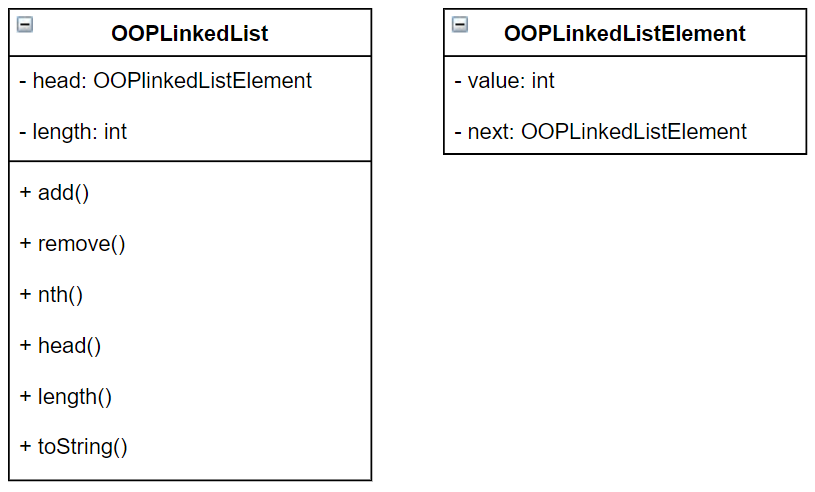
\includegraphics[scale=0.7]{UMLdiagram}
\end{center}
\end{enumerate}

\subsection*{5.5}
Implemented in ``OOPSortedLinkedList.java''. The code is pasted below.

\begin{verbatim}
package uk.ac.cam.hjel2.OOPsv1.LinkedList;

public class OOPSortedLinkedList extends OOPLinkedList{

    @Override
    public void add(int n){
        OOPLinkedListElement current = head;
        if (head == null || n < head.value){
            head = new OOPLinkedListElement(n, head);
        }
        else{
            insert(n, current, current.next);
        }
    }
	
    private void insert(int n, OOPLinkedListElement previous, OOPLinkedListElement current){
        if (current == null){
            previous.next = new OOPLinkedListElement(n, null);
            length++;
        }
        else if (n < current.value){
            previous.next = new OOPLinkedListElement(n, current);
            length++;
        }
        else{
            insert(n, current, current.next);
        }
    }
}
\end{verbatim}

\end{enumerate}

\end{document}

